\chapter*{Conclusion et perspectives}
\addcontentsline{toc}{chapter}{Conclusion}
\markboth{Conclusion}{Conclusion}
\label{sec:conclusion}


Une amélioration future plus qu'intéressante et déjà entamée par le groupe serait de changer la modélisation de notre jeu via Unity pour pouvoir y jouer avec une vue en 3D. Cette idée serait révolutionnaire pour changer le fait que le Pong ne peut se jouer que sur un plateau en 2D. Voici une brève représentation de ce que donnerait une modélisation de notre jeu sur Unity:

\begin{figure}[ht]
  \centering
  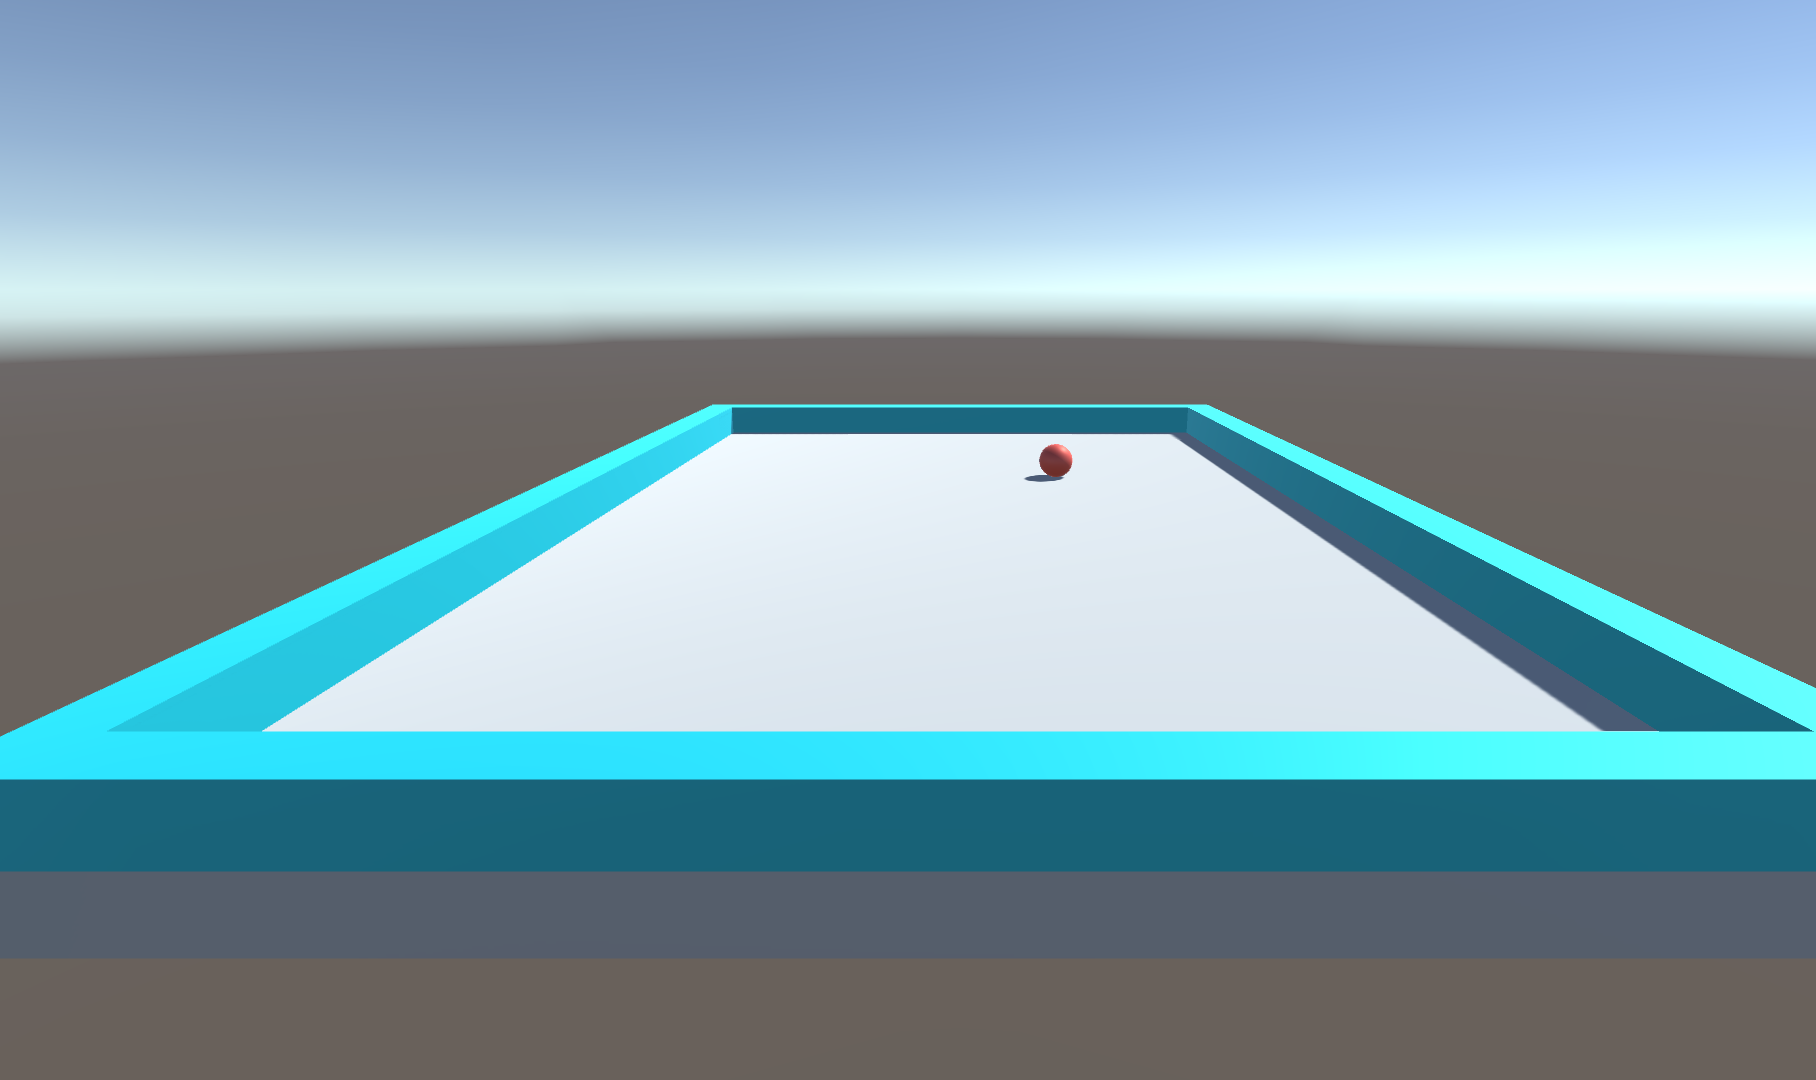
\includegraphics[width=5cm]{images/Capture12}
  \caption{Illustration de notre jeu sur Unity.}
  \label{fig:une-image}
\end{figure}

Cette amélioration nous inspire beaucoup pour l'avenir de notre jeu.\\
Pour conclure, Nous pouvons dire que ce projet fut très enrichissant pour chacun d'entre nous. D'ailleurs nous allons continuer a travailler dessus pour peut-être un jour le rendre public et collecter l'avis des joueurs sur notre vision d'un Pong moderne.